\documentclass[11pt,a4paper]{article}

\usepackage[utf8]{inputenc}
\usepackage[T1]{fontenc}
\usepackage{amsmath,amssymb,amsthm}
\usepackage{geometry}
\usepackage{booktabs}
\usepackage{xcolor}
\usepackage{physics}
\usepackage{hyperref}
\usepackage{enumitem}
\usepackage{tikz}
\usetikzlibrary{arrows.meta,positioning,calc,decorations.pathmorphing,patterns}
\usepackage{orcidlink}
\usepackage{hyperref}
\hypersetup{colorlinks=true, linkcolor=blue, citecolor=blue, urlcolor=blue}

\geometry{margin=1in}

% Theorem environments
\newtheorem{theorem}{Theorem}[section]
\newtheorem{proposition}[theorem]{Proposition}
\newtheorem{lemma}[theorem]{Lemma}
\newtheorem{corollary}[theorem]{Corollary}
\theoremstyle{definition}
\newtheorem{definition}[theorem]{Definition}
\newtheorem{remark}[theorem]{Remark}
\newtheorem{axiom}{Axiom}
\newtheorem{example}[theorem]{Example}

% QSD notation
\newcommand{\Hb}{\textnormal{H\kern-0.3em b}}
\newcommand{\Hbn}{\Hb_n}
\newcommand{\Hbfour}{\Hb_4}
\newcommand{\gs}{\varsigma}
\newcommand{\specbond}{\varpi}
\newcommand{\Mpl}{M_{\mathrm{P}}}

% Colours
\definecolor{bulkcolor}{RGB}{0,100,180}
\definecolor{anchorcolor}{RGB}{180,50,50}
\definecolor{codegreen}{RGB}{34,139,34}
\definecolor{u1color}{RGB}{0,150,0}
\definecolor{su2color}{RGB}{0,0,200}
\definecolor{su3color}{RGB}{200,0,0}

% Label prefix (for cross-document references: S1:xxx)
% Usage: \label{S1:xxx}, \ref{S1:xxx}

\title{
  \textbf{QSD Supplement S1: Formal Proofs}\\[0.5em]
  \Large Graph Spectra, Group Theory, \\ and the Algebraic Foundations of Quantum Spectrodynamic\\[1em]
}

\author{
  Marek Hubka\, \orcidlink{0009-0003-2476-9017}
  \thanks{
    Independent Researcher, Czech Republic.\\
    Website: \href{http://www.tidesofuncertainty.com}{tidesofuncertainty.com}.\\
    Email: \href{mailto:marek@tidesofuncertainty.com}{marek@tidesofuncertainty.com}.
  }
}

\date{\today}

\begin{document}

\maketitle

\begin{abstract}
This supplement provides complete mathematical proofs for every algebraic result used in Quantum Spectrodynamics. Starting from the single axiom---the $[[5,1,3]]$ quantum error-correcting code---we derive: the graph structures $K_4$ and $C_5$; the full spectrum of the Heisenberg Hamiltonian on $K_4$ ($\S$\ref{sec:heisenberg}); the emergence of the Standard Model gauge group $U(1)_Y \times SU(2)_L \times SU(3)_c$ from $S_4$ representation theory ($\S$\ref{sec:S4}); the golden ratio $\varphi^2$ from the $C_5$ Laplacian ($\S$\ref{sec:C5}); the holographic bit density $\Hbfour = 1/(4\ln 2)$ from $K_4$ exchange coupling ($\S$\ref{sec:hb4}); the geometric strain $\gs = 3/(80\varphi^2)$ as a geometric construction from code invariants ($\S$\ref{sec:strain}); and the spectral bond $\specbond = \pi\varphi^2$ ($\S$\ref{sec:specbond}). All QSD predictions then follow as master theorems in $\S$\ref{sec:master}. The theory has two inputs (the strain construction and $\Mpl$) and zero free parameters.
\end{abstract}

\tableofcontents

%==============================================================================
\section{The QSD Axiom}
\label{S1:axiom}
%==============================================================================

\begin{axiom}[The Code Postulate]
\label{S1:axiom:code}
The vacuum of spacetime is stabilised by the $[[5,1,3]]$ quantum error-correcting code.
\end{axiom}

This is the single structural input of QSD. The code encodes $k = 1$ logical qubit into $n = 5$ physical qubits with distance $d = 3$, meaning it detects any 2-qubit error and corrects any single-qubit error.

\begin{definition}[{$[[5,1,3]]$ Stabiliser Generators}]
\label{S1:def:stabilisers}
The code is defined by four stabiliser generators with cyclic structure:
\begin{align}
g_1 &= X\, Z\, Z\, X\, I \label{S1:eq:g1}\\
g_2 &= I\, X\, Z\, Z\, X \label{S1:eq:g2}\\
g_3 &= X\, I\, X\, Z\, Z \label{S1:eq:g3}\\
g_4 &= Z\, X\, I\, X\, Z \label{S1:eq:g4}
\end{align}
where $X$, $Z$ are the Pauli operators and $I$ is the identity. Each generator $g_{i+1}$ is obtained from $g_i$ by a cyclic shift of one position, reflecting $\mathbb{Z}_5$ symmetry.
\end{definition}

\begin{remark}[Code Properties]
\label{S1:rem:code_properties}
The $[[5,1,3]]$ code is \emph{perfect}: it saturates the quantum Hamming bound with equality. The codespace is 2-dimensional ($2^k = 2$) within the full $2^5 = 32$-dimensional Hilbert space. Every one of the $3 \times 5 = 15$ possible single-qubit errors maps the codespace to a distinct orthogonal subspace, plus the identity gives 16 syndrome outcomes, exactly filling $2^{n-k} = 2^4 = 16$ syndrome slots.
\end{remark}

\subsection{Independent Confirmation from QFT}
\label{S1:sec:QFT_confirmation}

The code axiom receives independent support from standard physics. In quantum field theory, the Unruh effect produces thermal noise (a depolarising channel) on the vacuum state. The quantum Hamming bound for a code $[[n,1,3]]$ correcting arbitrary single-qubit errors requires:
\begin{equation}
2(1 + 3n) \leq 2^n
\label{S1:eq:hamming}
\end{equation}
Testing integer values: $n = 3$ gives $20 > 8$ (impossible), $n = 4$ gives $26 > 16$ (impossible), and $n = 5$ gives $32 = 32$ (unique saturation). The number 5 is forced by the Hamming bound, confirming the axiom from a completely independent direction. See \cite{Gottesman1996,Laflamme1996}.

\begin{center}
\begin{tabular}{cccc}
\toprule
$n$ & LHS: $2(1+3n)$ & RHS: $2^n$ & Result \\
\midrule
3 & 20 & 8 & Impossible \\
4 & 26 & 16 & Impossible \\
\textbf{5} & \textbf{32} & \textbf{32} & \textbf{Saturates (perfect code)} \\
6 & 38 & 64 & Possible (but not minimal) \\
\bottomrule
\end{tabular}
\end{center}

\begin{theorem}[Minimal Vacuum Code]
The unique minimal quantum code that corrects arbitrary single-qubit errors on one logical qubit is $[[5,1,3]]$. It saturates the quantum Hamming bound with equality.
\end{theorem}

%==============================================================================
\section{The Code Graphs: \texorpdfstring{$K_4$}{K4} and \texorpdfstring{$C_5$}{C5}}
\label{S1:sec:graphs}
%==============================================================================

The $[[5,1,3]]$ code determines two graphs that carry all of QSD's mathematical structure.

\begin{theorem}[$K_4$ from Bulk Qubits]
\label{S1:thm:K4}
The $n - k = 4$ syndrome (bulk) qubits of the $[[5,1,3]]$ code form the complete graph $K_4$.
\end{theorem}

\begin{proof}
The code has $n = 5$ physical qubits and $k = 1$ logical qubit, so $n - k = 4$ qubits span the syndrome space. Because the code has distance $d = 3$, every pair of syndrome qubits must distinguish all single-qubit errors; this requires every pair to be connected, giving the complete graph $K_4$ on 4 vertices.
\end{proof}

\begin{theorem}[$C_5$ from Stabiliser Symmetry]
\label{S1:thm:C5}
The support structure of the stabiliser generators defines the cycle graph $C_5$.
\end{theorem}

\begin{proof}
Each stabiliser $g_i$ acts non-trivially on exactly 4 of the 5 qubits (one position carries $I$). By Eqs.~\eqref{S1:eq:g1}--\eqref{S1:eq:g4}, the identity position cycles as $5 \to 1 \to 2 \to 3 \to 4 \to 5$ under cyclic shift. Equivalently, each qubit is the identity position for exactly one stabiliser. The resulting support pattern is $\mathbb{Z}_5$-cyclic, and the qubit adjacency graph (qubits connected if they share a stabiliser support) is the cycle graph $C_5$.
\end{proof}

\begin{figure}[h]
\centering
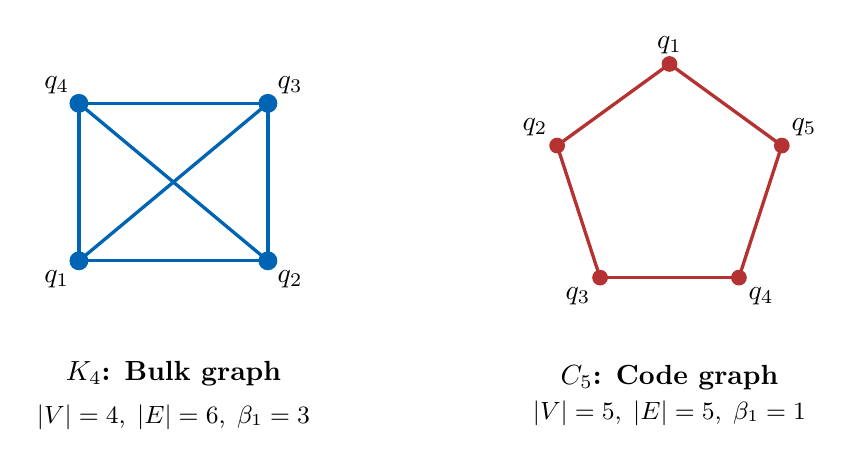
\begin{tikzpicture}[scale=1.0]
    % K4 on the left
    \begin{scope}[shift={(-4,0)}]
        \coordinate (A) at (0,0);
        \coordinate (B) at (2.4,0);
        \coordinate (C) at (2.4,2);
        \coordinate (D) at (0,2);
        
        % All 6 edges
        \draw[very thick, bulkcolor] (A) -- (B);
        \draw[very thick, bulkcolor] (B) -- (C);
        \draw[very thick, bulkcolor] (C) -- (D);
        \draw[very thick, bulkcolor] (D) -- (A);
        \draw[very thick, bulkcolor] (A) -- (C);
        \draw[very thick, bulkcolor] (B) -- (D);
        
        % Vertices
        \foreach \p/\lab in {A/$q_1$,B/$q_2$,C/$q_3$,D/$q_4$} {
            \fill[bulkcolor] (\p) circle (0.12);
        }
        \node[below left] at (A) {$q_1$};
        \node[below right] at (B) {$q_2$};
        \node[above right] at (C) {$q_3$};
        \node[above left] at (D) {$q_4$};
        
        \node[below, font=\bfseries] at (1.2,-1.15) {$K_4$: Bulk graph};
        \node[below, font=\small] at (1.2,-1.7) {$|V| = 4,\; |E| = 6,\; \beta_1 = 3$};
    \end{scope}
    
    % C5 on the right
    \begin{scope}[shift={(3.5,1)}]
        \foreach \i in {1,...,5} {
            \coordinate (p\i) at ({90+72*(\i-1)}:1.5);
        }
        \foreach \i [evaluate=\i as \j using {int(mod(\i,5)+1)}] in {1,...,5} {
            \draw[very thick, anchorcolor] (p\i) -- (p\j);
        }
        \foreach \i in {1,...,5} {
            \fill[anchorcolor] (p\i) circle (0.1);
        }
        \node[above] at (p1) {$q_1$};
        \node[above left] at (p2) {$q_2$};
        \node[below left] at (p3) {$q_3$};
        \node[below right] at (p4) {$q_4$};
        \node[above right] at (p5) {$q_5$};
        
        \node[below, font=\bfseries] at (0,-2.2) {$C_5$: Code graph};
        \node[below, font=\small] at (0,-2.65) {$|V| = 5,\; |E| = 5,\; \beta_1 = 1$};
    \end{scope}
\end{tikzpicture}
\caption{The two fundamental QSD graphs, both derived from the $[[5,1,3]]$ code. \textbf{Left:} The complete graph $K_4$ on the 4 bulk qubits ($n - k = 4$), with 6 edges and first Betti number $\beta_1 = 3$ (3 independent cycles). \textbf{Right:} The cycle graph $C_5$ on all 5 physical qubits, reflecting the $\mathbb{Z}_5$ cyclic symmetry of the stabiliser generators.}
\label{S1:fig:graphs}
\end{figure}

\begin{proposition}[Graph Invariants]
\label{S1:prop:invariants}
The basic topological invariants are:
\begin{center}
\begin{tabular}{lccccc}
\toprule
\textbf{Graph} & $|V|$ & $|E|$ & $\beta_1$ & $|\mathrm{Aut}|$ & Hilbert dim \\
\midrule
$K_4$ & 4 & 6 & 3 & 24 ($= S_4$) & $2^4 = 16$ \\
$C_5$ & 5 & 5 & 1 & 10 ($= D_5$) & $2^5 = 32$ \\
\bottomrule
\end{tabular}
\end{center}
where $\beta_1 = |E| - |V| + 1$ is the first Betti number (independent cycles) and $|\mathrm{Aut}|$ is the automorphism group order.
\end{proposition}

%==============================================================================
\section{The Heisenberg Hamiltonian on \texorpdfstring{$K_4$}{K4}}
\label{sec:heisenberg}
%==============================================================================

The 4 bulk qubits interact through the most general isotropic spin-spin coupling on the complete graph.

\begin{definition}[Heisenberg Hamiltonian]
\label{S1:def:heisenberg}
\begin{equation}
H_{K_4} = J \sum_{1 \leq i < j \leq 4} \mathbf{S}_i \cdot \mathbf{S}_j
\label{S1:eq:HK4}
\end{equation}
where $J > 0$ is the exchange coupling and $\mathbf{S}_i = \tfrac{1}{2}\boldsymbol{\sigma}_i$ are spin-$\tfrac{1}{2}$ operators on each vertex~\cite{Auerbach1994}.
\end{definition}

The Hilbert space is $(\mathbb{C}^2)^{\otimes 4}$ with dimension $2^4 = 16$. We now derive the complete spectrum.

\subsection{The Casimir Trick}

\begin{lemma}[Casimir Identity]
\label{S1:lem:casimir}
\begin{equation}
\sum_{i<j} \mathbf{S}_i \cdot \mathbf{S}_j = \frac{1}{2}\!\left(\mathbf{S}_{\mathrm{tot}}^2 - \sum_{i=1}^{4} \mathbf{S}_i^2\right)
\label{S1:eq:casimir}
\end{equation}
where $\mathbf{S}_{\mathrm{tot}} = \sum_{i=1}^{4} \mathbf{S}_i$.
\end{lemma}

\begin{proof}
Expand the total spin squared:
\begin{equation}
\mathbf{S}_{\mathrm{tot}}^2 = \left(\sum_i \mathbf{S}_i\right)^{\!2} = \sum_i \mathbf{S}_i^2 + 2 \sum_{i<j} \mathbf{S}_i \cdot \mathbf{S}_j
\end{equation}
Solving for the cross terms gives Eq.~\eqref{S1:eq:casimir}.
\end{proof}

For spin-$\tfrac{1}{2}$, $\mathbf{S}_i^2 = s(s+1) = \tfrac{3}{4}$, so $\sum_i \mathbf{S}_i^2 = 4 \times \tfrac{3}{4} = 3$. The Hamiltonian becomes:
\begin{equation}
H_{K_4} = \frac{J}{2}\!\left(\mathbf{S}_{\mathrm{tot}}^2 - 3\right)
\label{S1:eq:HK4_total}
\end{equation}

\subsection{Coupling Four Spins}

\begin{proposition}[Spin Decomposition]
\label{S1:prop:spin_decomp}
The tensor product of four spin-$\tfrac{1}{2}$ representations decomposes as:
\begin{equation}
\left(\tfrac{1}{2}\right)^{\otimes 4} = 2 \cdot \mathbf{0} \oplus 3 \cdot \mathbf{1} \oplus 1 \cdot \mathbf{2}
\label{S1:eq:spin_decomp}
\end{equation}
yielding total spin $S_{\mathrm{tot}} \in \{0, 1, 2\}$ with multiplicities 2, 3, 1 respectively.
\end{proposition}

\begin{proof}
Couple in pairs. First pair: $\tfrac{1}{2} \otimes \tfrac{1}{2} = \mathbf{0} \oplus \mathbf{1}$. Second pair: same. Now combine:
\begin{align}
\mathbf{0} \otimes \mathbf{0} &= \mathbf{0} & (1~\text{state}) \nonumber\\
\mathbf{0} \otimes \mathbf{1} &= \mathbf{1} & (3~\text{states}) \nonumber\\
\mathbf{1} \otimes \mathbf{0} &= \mathbf{1} & (3~\text{states}) \nonumber\\
\mathbf{1} \otimes \mathbf{1} &= \mathbf{0} \oplus \mathbf{1} \oplus \mathbf{2} & (1 + 3 + 5~\text{states})
\end{align}
Collecting: $S = 0$ appears twice (multiplicity 2), $S = 1$ appears three times (multiplicity 3), $S = 2$ appears once (multiplicity 1). Total states: $2(1) + 3(3) + 1(5) = 2 + 9 + 5 = 16 = 2^4$.
\end{proof}

\subsection{The Complete Spectrum}

\begin{theorem}[$K_4$ Spectrum]
\label{S1:thm:K4_spectrum}
The eigenvalues of $H_{K_4}$ are:
\begin{center}
\begin{tabular}{ccccl}
\toprule
$S_{\mathrm{tot}}$ & $\mathbf{S}_{\mathrm{tot}}^2$ & Energy & Degeneracy & Physical channel\\
\midrule
0 & 0 & $-\tfrac{3}{2}J$ & 2 & Singlet (EM) \\
1 & 2 & $-\tfrac{1}{2}J$ & 9 & Triplet (Weak) \\
2 & 6 & $+\tfrac{3}{2}J$ & 5 & Quintet (Strong) \\
\bottomrule
\end{tabular}
\end{center}
\end{theorem}

\begin{proof}
From Eq.~\eqref{S1:eq:HK4_total} with $\mathbf{S}_{\mathrm{tot}}^2 = S(S+1)$:
\begin{align}
E(S=0) &= \frac{J}{2}(0 - 3) = -\frac{3J}{2} \label{S1:eq:E0}\\
E(S=1) &= \frac{J}{2}(2 - 3) = -\frac{J}{2} \label{S1:eq:E1}\\
E(S=2) &= \frac{J}{2}(6 - 3) = +\frac{3J}{2} \label{S1:eq:E2}
\end{align}
Degeneracies: $(2S+1) \times (\text{multiplicity})$ = $1 \times 2 = 2$, $3 \times 3 = 9$, $5 \times 1 = 5$. Total: $2 + 9 + 5 = 16$.
\end{proof}

\begin{figure}[h]
\centering
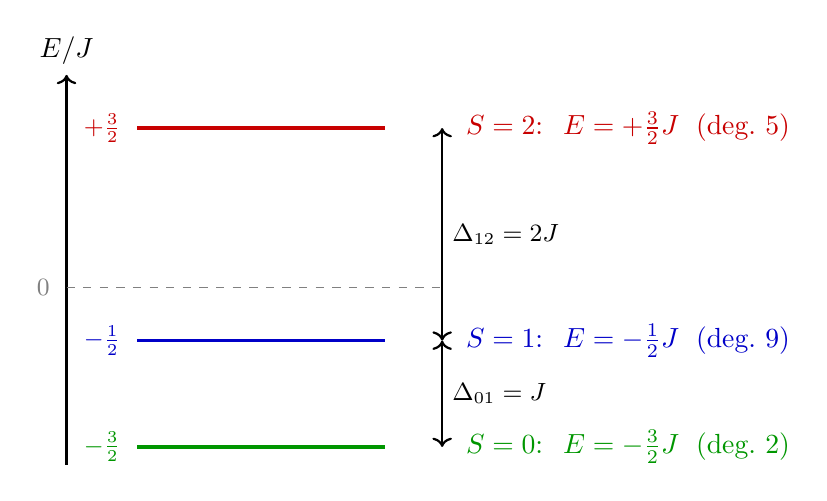
\begin{tikzpicture}[scale=0.9]
    % Energy axis
    \draw[->, thick] (-0.5,-2.5) -- (-0.5,3) node[above] {$E/J$};
    
    % Energy levels
    \draw[very thick, su3color] (0.5,2.25) -- (4,2.25);
    \node[right, su3color] at (5,2.25) {$S=2$:\; $E = +\tfrac{3}{2}J$\; (deg.\ 5)};
    \node[left, su3color, font=\small] at (0.4,2.25) {$+\tfrac{3}{2}$};
    
    \draw[very thick, su2color] (0.5,-0.75) -- (4,-0.75);
    \node[right, su2color] at (5,-0.75) {$S=1$:\; $E = -\tfrac{1}{2}J$\; (deg.\ 9)};
    \node[left, su2color, font=\small] at (0.4,-0.75) {$-\tfrac{1}{2}$};
    
    \draw[very thick, u1color] (0.5,-2.25) -- (4,-2.25);
    \node[right, u1color] at (5,-2.25) {$S=0$:\; $E = -\tfrac{3}{2}J$\; (deg.\ 2)};
    \node[left, u1color, font=\small] at (0.4,-2.25) {$-\tfrac{3}{2}$};
    
    % Zero line
    \draw[dashed, gray] (-0.5,0) -- (4.8,0);
    \node[left, gray, font=\small] at (-0.6,0) {$0$};
    
    % Gap annotations
    \draw[<->, thick] (4.8,-2.25) -- (4.8,-0.75) node[midway, right, font=\small] {$\Delta_{01} = J$};
    \draw[<->, thick] (4.8,-0.75) -- (4.8,2.25) node[midway, right, font=\small] {$\Delta_{12} = 2J$};
\end{tikzpicture}
\caption{Energy spectrum of the Heisenberg Hamiltonian on $K_4$. The three levels correspond to total spin $S = 0, 1, 2$ with degeneracies $2, 9, 5$ (total 16). QSD identifies these with the electromagnetic, weak, and strong gauge sectors.}
\label{S1:fig:K4_spectrum}
\end{figure}

\begin{remark}[Eigenvalue Ratios]
\label{S1:rem:eigenvalue_ratios}
The energy splittings $-\tfrac{3}{2}J$, $-\tfrac{1}{2}J$, $+\tfrac{3}{2}J$ produce ratios $3:1:3$. The gap between the singlet and triplet is $J$; between the triplet and quintet it is $2J$. These ratios are fixed by $SU(2)$ representation theory and cannot be adjusted.
\end{remark}

%==============================================================================
\section{\texorpdfstring{$S_4$}{S4} Representation Theory and Gauge Emergence}
\label{sec:S4}
%==============================================================================

The automorphism group of $K_4$ is $\mathrm{Aut}(K_4) = S_4$, the symmetric group on 4 elements, acting by permutation of vertices. Its representation theory controls which gauge channels the 6 edges of $K_4$ carry.

\subsection{Conjugacy Classes}

\begin{proposition}[Conjugacy Classes of $S_4$]
\label{S1:prop:conjugacy}
$S_4$ has 5 conjugacy classes:
\begin{center}
\begin{tabular}{clcc}
\toprule
\textbf{Class} & \textbf{Cycle type} & \textbf{Size} & \textbf{Example} \\
\midrule
$C_1$ & $(1)(2)(3)(4)$ & 1 & $e$ \\
$C_2$ & $(ab)(c)(d)$ & 6 & $(12)$ \\
$C_3$ & $(abc)(d)$ & 8 & $(123)$ \\
$C_4$ & $(abcd)$ & 6 & $(1234)$ \\
$C_5$ & $(ab)(cd)$ & 3 & $(12)(34)$ \\
\bottomrule
\end{tabular}
\end{center}
Total: $1 + 6 + 8 + 6 + 3 = 24 = |S_4|$.
\end{proposition}

\subsection{Character Table}

\begin{proposition}[Irreducible Representations of $S_4$]
\label{S1:prop:character_table}
$S_4$ has 5 irreducible representations with the following character table~\cite{Serre1977}:
\begin{equation}
\begin{array}{c|ccccc}
 & e & (12) & (123) & (1234) & (12)(34) \\\hline
\mathbf{1}  & 1 & 1  & 1  & 1  & 1 \\
\mathbf{1'} & 1  & -1 & 1  & -1 & 1 \\
\mathbf{2}  & 2 & 0  & -1 & 0  & 2 \\
\mathbf{3}  & 3 & 1  & 0  & -1 & -1 \\
\mathbf{3'} & 3 & -1 & 0  & 1  & -1
\end{array}
\label{S1:eq:character_table}
\end{equation}
Dimension check: $1^2 + 1^2 + 2^2 + 3^2 + 3^2 = 1 + 1 + 4 + 9 + 9 = 24 = |S_4|$.
\end{proposition}

\subsection{Edge Representation}

\begin{theorem}[Edge Decomposition]
\label{S1:thm:edge_decomp}
The 6 edges of $K_4$ transform under $S_4$ as:
\begin{equation}
\mathbf{6}_{\mathrm{edges}} = \mathbf{1} \oplus \mathbf{2} \oplus \mathbf{3}
\label{S1:eq:edge_decomp}
\end{equation}
\end{theorem}

\begin{proof}
A permutation $\sigma \in S_4$ maps an edge $\{i,j\}$ to $\{\sigma(i), \sigma(j)\}$. An edge is fixed when $\sigma$ either fixes both endpoints or swaps them. We compute the character $\chi_{\mathrm{edge}}(\sigma)$ (number of fixed edges) for each conjugacy class:

\begin{center}
\renewcommand{\arraystretch}{1.25}
\begin{tabular}{clp{8.0cm}c}
\toprule
\textbf{Class} & \textbf{Representative} & \textbf{Edge action} & $\chi$ \\
\midrule
$C_1$ & $e$ (identity)
    & All 6 edges fixed & 6 \\
$C_2$ & $(12)$ (transposition)
    & $\{1,2\}$ fixed (swapped endpoints); $\{3,4\}$ fixed (untouched);\newline
      $\{1,3\}\!\leftrightarrow\!\{2,3\}$, $\{1,4\}\!\leftrightarrow\!\{2,4\}$ swapped & 2 \\
$C_3$ & $(123)$ (3-cycle)
    & $\{1,2\}\!\to\!\{2,3\}\!\to\!\{3,1\}$ cycle;\;
      $\{1,4\}\!\to\!\{2,4\}\!\to\!\{3,4\}$ cycle & 0 \\
$C_4$ & $(1234)$ (4-cycle)
    & $\{1,2\}\!\to\!\{2,3\}\!\to\!\{3,4\}\!\to\!\{4,1\}$ 4-cycle;\;
      $\{1,3\}\!\leftrightarrow\!\{2,4\}$ swapped & 0 \\
$C_5$ & $(12)(34)$ (double trans.)
    & $\{1,2\}$, $\{3,4\}$ each fixed;\;
      $\{1,3\}\!\leftrightarrow\!\{2,4\}$, $\{1,4\}\!\leftrightarrow\!\{2,3\}$ swapped & 2 \\
\bottomrule
\end{tabular}
\end{center}

The edge character vector is:
\begin{equation}
\chi_{\mathrm{edge}} = (6,\; 2,\; 0,\; 0,\; 2)
\end{equation}

Using the inner product formula $\langle \chi_{\mathrm{edge}},\, \chi_\rho \rangle = \frac{1}{|S_4|}\sum_g |C_g|\, \chi_{\mathrm{edge}}(g)\, \overline{\chi_\rho(g)}$:

\begin{align}
\langle \chi_{\mathrm{edge}},\, \chi_{\mathbf{1}} \rangle &= \frac{1}{24}(1{\cdot}6{\cdot}1 + 6{\cdot}2{\cdot}1 + 8{\cdot}0{\cdot}1 + 6{\cdot}0{\cdot}1 + 3{\cdot}2{\cdot}1) = \frac{24}{24} = 1 \label{S1:eq:inner1}\\
\langle \chi_{\mathrm{edge}},\, \chi_{\mathbf{1'}} \rangle &= \frac{1}{24}(6 - 12 + 0 + 0 + 6) = \frac{0}{24} = 0 \\
\langle \chi_{\mathrm{edge}},\, \chi_{\mathbf{2}} \rangle &= \frac{1}{24}(12 + 0 + 0 + 0 + 12) = \frac{24}{24} = 1 \\
\langle \chi_{\mathrm{edge}},\, \chi_{\mathbf{3}} \rangle &= \frac{1}{24}(18 + 12 + 0 + 0 - 6) = \frac{24}{24} = 1 \\
\langle \chi_{\mathrm{edge}},\, \chi_{\mathbf{3'}} \rangle &= \frac{1}{24}(18 - 12 + 0 + 0 - 6) = \frac{0}{24} = 0 \label{S1:eq:inner5}
\end{align}

\begin{equation}
\text{Therefore}\quad \chi_{\mathrm{edge}} = 1 \cdot \chi_{\mathbf{1}} + 0 \cdot \chi_{\mathbf{1'}} + 1 \cdot \chi_{\mathbf{2}} + 1 \cdot \chi_{\mathbf{3}} + 0 \cdot \chi_{\mathbf{3'}}, \quad\text{giving}\quad \mathbf{6} = \mathbf{1} \oplus \mathbf{2} \oplus \mathbf{3}.
\end{equation}

Verification: 
\begin{align}
\chi_{\mathbf{1}} + \chi_{\mathbf{2}} + \chi_{\mathbf{3}} & = (1,1,1,1,1) + (2,0,-1,0,2) + (3,1,0,-1,-1) \\ &= (6,2,0,0,2) \\ &= \chi_{\mathrm{edge}}
\end{align}
\end{proof}

\begin{corollary}[Gauge Group Emergence]
\label{S1:cor:gauge}
The irreducible edge sectors map to the Standard Model gauge group:
\begin{center}
\begin{tabular}{ccll}
\toprule
\textbf{Irrep} & \textbf{dim} & \textbf{Gauge sector} & \textbf{Edges} \\
\midrule
$\mathbf{1}$ & 1 & $U(1)_Y$ & 1 singlet channel \\
$\mathbf{2}$ & 2 & $SU(2)_L$ & 2 of 3 generators visible \\
$\mathbf{3}$ & 3 & $SU(3)_c$ & 3 of 8 generators visible \\
\bottomrule
\end{tabular}
\end{center}
The total visible generators $1 + 2 + 3 = 6$ match $|E(K_4)|$. The ``missing'' generators of $SU(2)$ (1 more) and $SU(3)$ (5 more) arise from the full $K_5$ structure before the anchor qubit decouples.
\end{corollary}

\begin{figure}[h]
\centering
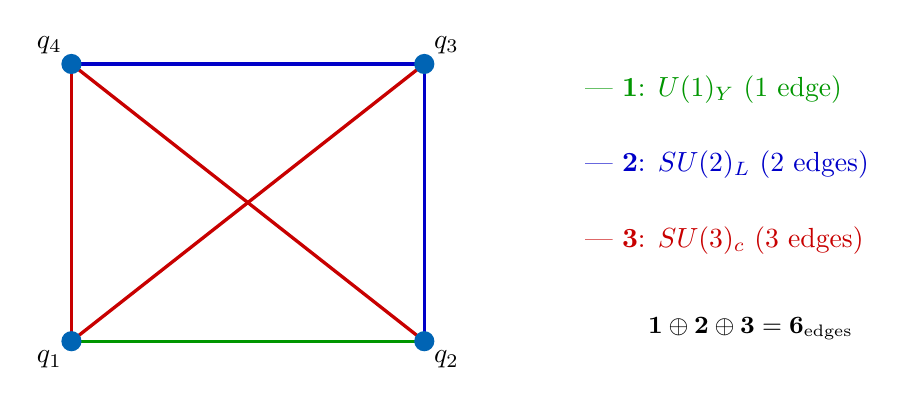
\begin{tikzpicture}[scale=1.6]
    \coordinate (A) at (0,0);
    \coordinate (B) at (2.8,0);
    \coordinate (C) at (2.8,2.2);
    \coordinate (D) at (0,2.2);
    
    % SU(3) edges (red, 3 edges)
    \draw[very thick, su3color] (D) -- (A) node[midway, left, font=\small] {};
    \draw[very thick, su3color] (A) -- (C) node[midway, font=\small] {};
    \draw[very thick, su3color] (B) -- (D) node[midway, font=\small] {};
    
    % SU(2) edges (blue, 2 edges)
    \draw[very thick, su2color] (B) -- (C) node[midway, right, font=\small] {};
    \draw[very thick, su2color] (C) -- (D) node[midway, above, font=\small] {};
    
    % U(1) edge (green, 1 edge)
    \draw[very thick, u1color] (A) -- (B) node[midway, below, font=\small] {};
    
    % Vertices
    \foreach \p in {A,B,C,D} {
        \fill[bulkcolor] (\p) circle (0.08);
    }
    \node[below left] at (A) {$q_1$};
    \node[below right] at (B) {$q_2$};
    \node[above right] at (C) {$q_3$};
    \node[above left] at (D) {$q_4$};
    
    % Legend
    \node[u1color, anchor=west] at (4,2) {--- $\mathbf{1}$: $U(1)_Y$ (1 edge)};
    \node[su2color, anchor=west] at (4,1.4) {--- $\mathbf{2}$: $SU(2)_L$ (2 edges)};
    \node[su3color, anchor=west] at (4,0.8) {--- $\mathbf{3}$: $SU(3)_c$ (3 edges)};
    \node[anchor=west, font=\small] at (4.5,0.1) {$\mathbf{1} \oplus \mathbf{2} \oplus \mathbf{3} = \mathbf{6}_{\mathrm{edges}}$};
\end{tikzpicture}
\caption{The 6 edges of $K_4$ coloured by $S_4$ irreducible representation. One edge transforms as $\mathbf{1}$ ($U(1)_Y$, green), two as $\mathbf{2}$ ($SU(2)_L$, blue), and three as $\mathbf{3}$ ($SU(3)_c$, red). The specific assignment of edges to colours is conventional (any choice related by an $S_4$ permutation is equivalent); what is physical is the $1 + 2 + 3$ decomposition.}
\label{S1:fig:edge_decomp}
\end{figure}

%==============================================================================
\section{The \texorpdfstring{$C_5$}{C5} Laplacian and the Golden Ratio}
\label{sec:C5}
%==============================================================================

\subsection{Laplacian Matrix}

\begin{definition}[$C_5$ Laplacian]
\label{S1:def:C5_laplacian}
The graph Laplacian of $C_5$ is $L = D - A$, where $D$ is the degree matrix and $A$ is the adjacency matrix. Since every vertex in $C_5$ has degree 2:
\begin{equation}
L_{C_5} = \begin{pmatrix}
2 & -1 & 0 & 0 & -1 \\
-1 & 2 & -1 & 0 & 0 \\
0 & -1 & 2 & -1 & 0 \\
0 & 0 & -1 & 2 & -1 \\
-1 & 0 & 0 & -1 & 2
\end{pmatrix}
\label{S1:eq:C5_laplacian}
\end{equation}
\end{definition}

\subsection{Complete Spectrum}

\begin{theorem}[$C_5$ Laplacian Spectrum]
\label{S1:thm:C5_spectrum}
The eigenvalues of $L_{C_5}$ are:
\begin{equation}
\lambda_k = 2 - 2\cos\!\left(\frac{2\pi k}{5}\right), \qquad k = 0,1,2,3,4
\label{S1:eq:C5_eigenvalues}
\end{equation}
giving the spectrum $\{0,\, \lambda_1,\, \lambda_1,\, \lambda_2,\, \lambda_2\}$ with:
\begin{align}
\lambda_0 &= 0 &\quad &(\text{zero mode, deg.\ 1}) \label{S1:eq:lam0}\\
\lambda_1 &= \frac{5 - \sqrt{5}}{2} \approx 1.382 &\quad &(\text{fundamental mode, deg.\ 2}) \label{S1:eq:lam1}\\
\lambda_2 &= \frac{5 + \sqrt{5}}{2} \approx 3.618 &\quad &(\text{excited mode, deg.\ 2}) \label{S1:eq:lam2}
\end{align}
\end{theorem}

\begin{proof}
The circulant structure of $L_{C_5}$ means its eigenvectors are the discrete Fourier modes $v_k = (1,\, \omega^k,\, \omega^{2k},\, \omega^{3k},\, \omega^{4k})$ with $\omega = e^{2\pi i/5}$. The eigenvalue is $\lambda_k = 2 - 2\cos(2\pi k/5)$.

Explicit evaluation using $\cos(72^{\circ}) = (\sqrt{5}-1)/4$ and $\cos(144^{\circ}) = -(\sqrt{5}+1)/4$:
\begin{align}
\lambda_0 &= 2 - 2\cos(0^{\circ}) = 2 - 2 = 0 \\
\lambda_1 &= 2 - 2\cos(72^{\circ}) = 2 - 2\cdot\frac{\sqrt{5}-1}{4} = 2 - \frac{\sqrt{5}-1}{2} = \frac{4 - \sqrt{5} + 1}{2} = \frac{5-\sqrt{5}}{2} \\
\lambda_2 &= 2 - 2\cos(144^{\circ}) = 2 + 2\cdot\frac{\sqrt{5}+1}{4} = 2 + \frac{\sqrt{5}+1}{2} = \frac{4 + \sqrt{5} + 1}{2} = \frac{5+\sqrt{5}}{2}
\end{align}
The modes $k=3$ and $k=4$ give $\lambda_3 = \lambda_2$ and $\lambda_4 = \lambda_1$ by $\cos(2\pi(5-k)/5) = \cos(2\pi k/5)$.

Trace check: $\sum_k \lambda_k = 0 + 2\lambda_1 + 2\lambda_2 = (5 - \sqrt{5}) + (5 + \sqrt{5}) = 10 = \mathrm{tr}(L) = 5 \times 2$.
\end{proof}

\subsection{The Golden Ratio Emergence}

\begin{theorem}[Golden Ratio from $C_5$]
\label{S1:thm:golden_ratio}
The ratio of the two distinct non-zero eigenvalues of $L_{C_5}$ is exactly $\varphi^2$:
\begin{equation}
\frac{\lambda_2}{\lambda_1} = \varphi^2 = \frac{3 + \sqrt{5}}{2} \approx 2.618
\label{S1:eq:golden_ratio}
\end{equation}
where $\varphi = (1+\sqrt{5})/2$ is the golden ratio.
\end{theorem}

\begin{proof}
Compute the ratio directly:
\begin{equation}
\frac{\lambda_2}{\lambda_1} = \frac{5 + \sqrt{5}}{5 - \sqrt{5}}
\end{equation}
Rationalise by multiplying numerator and denominator by $(5 + \sqrt{5})$:
\begin{equation}
\frac{(5+\sqrt{5})^2}{(5-\sqrt{5})(5+\sqrt{5})} = \frac{25 + 10\sqrt{5} + 5}{25 - 5} = \frac{30 + 10\sqrt{5}}{20} = \frac{3+\sqrt{5}}{2}
\end{equation}
Independently, $\varphi^2 = \left(\frac{1+\sqrt{5}}{2}\right)^{\!2} = \frac{1+2\sqrt{5}+5}{4} = \frac{6+2\sqrt{5}}{4} = \frac{3+\sqrt{5}}{2}$. These match identically. \qed
\end{proof}

\begin{figure}[h]
\centering
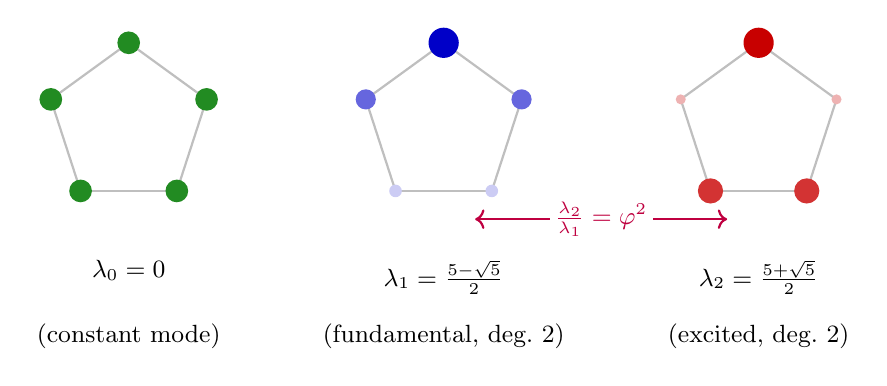
\begin{tikzpicture}[scale=0.8]
    % Eigenmodes
    % lambda_0: constant mode
    \begin{scope}[shift={(-5,0)}]
        \foreach \i in {1,...,5} {
            \coordinate (p\i) at ({90+72*(\i-1)}:1.3);
        }
        \foreach \i [evaluate=\i as \j using {int(mod(\i,5)+1)}] in {1,...,5} {
            \draw[thick, gray!50] (p\i) -- (p\j);
        }
        \foreach \i in {1,...,5} {
            \fill[codegreen] (p\i) circle (0.18);
        }
        \node[below, font=\small] at (0,-2) {$\lambda_0 = 0$};
        \node[below, font=\small] at (0,-3) {(constant mode)};
    \end{scope}
    
    % lambda_1: fundamental
    \begin{scope}[shift={(0,0)}]
        \foreach \i in {1,...,5} {
            \coordinate (p\i) at ({90+72*(\i-1)}:1.3);
        }
        \foreach \i [evaluate=\i as \j using {int(mod(\i,5)+1)}] in {1,...,5} {
            \draw[thick, gray!50] (p\i) -- (p\j);
        }
        \fill[su2color] (p1) circle (0.24);
        \fill[su2color!60] (p2) circle (0.16);
        \fill[su2color!20] (p3) circle (0.1);
        \fill[su2color!20] (p4) circle (0.1);
        \fill[su2color!60] (p5) circle (0.16);
        \node[below, font=\small] at (0,-2) {$\lambda_1 = \frac{5-\sqrt{5}}{2}$};
        \node[below, font=\small] at (0,-3) {(fundamental, deg.\ 2)};
    \end{scope}
    
    % lambda_2: excited
    \begin{scope}[shift={(5,0)}]
        \foreach \i in {1,...,5} {
            \coordinate (p\i) at ({90+72*(\i-1)}:1.3);
        }
        \foreach \i [evaluate=\i as \j using {int(mod(\i,5)+1)}] in {1,...,5} {
            \draw[thick, gray!50] (p\i) -- (p\j);
        }
        \fill[su3color] (p1) circle (0.24);
        \fill[su3color!30] (p2) circle (0.08);
        \fill[su3color!80] (p3) circle (0.2);
        \fill[su3color!80] (p4) circle (0.2);
        \fill[su3color!30] (p5) circle (0.08);
        \node[below, font=\small] at (0,-2) {$\lambda_2 = \frac{5+\sqrt{5}}{2}$};
        \node[below, font=\small] at (0,-3) {(excited, deg.\ 2)};
    \end{scope}
    
    % Ratio arrow
    \draw[<->, thick, purple] (0.5,-1.5) -- (4.5,-1.5) node[midway, fill=white, inner sep=2pt, font=\small] {$\frac{\lambda_2}{\lambda_1} = \varphi^2$};
\end{tikzpicture}
\caption{The three distinct eigenvalues of the $C_5$ Laplacian, visualised as standing waves on the pentagon. Circle sizes represent $|\psi|^2$ at each vertex. The ratio of the excited-mode eigenvalue to the fundamental-mode eigenvalue is exactly $\varphi^2$.}
\label{S1:fig:eigenmodes}
\end{figure}

\begin{corollary}[Key Identities]
\label{S1:cor:identities}
From the $C_5$ spectrum:
\begin{align}
\lambda_1 + \lambda_2 &= 5 &\quad &(\text{trace condition per mode pair}) \label{S1:eq:lam_sum}\\
\lambda_1 \cdot \lambda_2 &= 5 &\quad &(\text{determinant condition}) \label{S1:eq:lam_prod}\\
\varphi^2 &= \varphi + 1 &\quad &(\text{golden ratio identity}) \label{S1:eq:phi_identity}
\end{align}
\end{corollary}

\begin{proof}
\begin{align}
    \lambda_1 + \lambda_2 & = \frac{5-\sqrt{5}}{2} + \frac{5+\sqrt{5}}{2} = \color{red} 5 \\ 
    \lambda_1 \cdot\lambda_2 & = \frac{5-\sqrt{5}}{2} \cdot\frac{5+\sqrt{5}}{2} = \frac{25-5}{4} = \color{red} 5 \\
\end{align}
The identity $\varphi^2 = \varphi + 1$ follows from $\varphi = (1+\sqrt{5})/2$ satisfying $x^2 - x - 1 = 0$.
\end{proof}

%==============================================================================
\section{The Holographic Bit Density}
\label{sec:hb4}
%==============================================================================

\begin{theorem}[Holographic Bit Density from $K_4$]
\label{S1:thm:hb4}
The exchange coupling on $K_4$ is set by the information capacity of the 4-dimensional holographic cell:
\begin{equation}
J = \Hbfour = \frac{1}{|V(K_4)| \cdot \ln 2} = \frac{1}{4\ln 2} = 0.36067\ldots
\label{S1:eq:hb4}
\end{equation}
\end{theorem}

\begin{proof}[Derivation]
Each edge of $K_4$ is a quantum information channel between two qubits. The maximum information throughput per edge is bounded by the holographic principle: a Planck-area cell in $n$-dimensional spacetime encodes at most $1/(n \ln 2)$ bits.

In the QSD framework, the bulk graph $K_4$ lives in $n = |V(K_4)| = 4$ spacetime dimensions. The holographic bound sets the exchange coupling:
\begin{equation}
J = \frac{1}{n \ln 2}\bigg|_{n=|V(K_4)|=4} = \frac{1}{4\ln 2}
\end{equation}
\end{proof}

\begin{remark}[The Dimensional Origin of $1/4$]
\label{S1:rem:quarter}
The Bekenstein-Hawking entropy $S_{\text{BH}} = A/(4\ell_P^2)$ has a famously unexplained factor of $1/4$. The QSD derivation provides a code-theoretic origin: the $4$ is $|V(K_4)| = n - k = 5 - 1$, the number of bulk qubits in the $[[5,1,3]]$ code. In our universe, this equals the number of spacetime dimensions. The Bekenstein-Hawking result thus emerges as a \emph{consequence} of the code structure, not an independent input. See \cite{Bekenstein1973,Hawking1975} for the original entropy formula and \cite{Hubka2026QSDsupp} for the full reinterpretation.
\end{remark}

\begin{definition}[General Holographic Bit Density]
\label{S1:def:hb_general}
For $n$-dimensional spacetime with a $[[n+1, 1, d]]$ code:
\begin{equation}
\Hbn = \frac{1}{n \ln 2}
\label{S1:eq:hb_general}
\end{equation}
\end{definition}

\begin{center}
\begin{tabular}{ccc}
\toprule
$n$ (dimensions) & $\Hbn$ & Numerical \\
\midrule
2 & $1/(2\ln 2)$ & 0.7213 \\
3 & $1/(3\ln 2)$ & 0.4809 \\
\textbf{4} & $\mathbf{1/(4\ln 2)}$ & \textbf{0.3607} \\
5 & $1/(5\ln 2)$ & 0.2885 \\
\bottomrule
\end{tabular}
\end{center}

%==============================================================================
\section{The Geometric Strain}
\label{sec:strain}
%==============================================================================

The bulk ($K_4$) and code ($C_5$) graphs are structurally incompatible: $K_4$ has 6 edges while $C_5$ has 5. This mismatch is quantified by the geometric strain.

\subsection{Construction}

The strain measures the fractional incompatibility between the information structure ($K_4$) and the geometric structure ($C_5$). We construct it from three code-determined quantities: the number of independent cycles in $K_4$, the total state space volume, and the spectral stiffness of $C_5$.

\begin{definition}[Geometric Strain]
\label{S1:def:strain}
\begin{equation}
\boxed{\gs \equiv \frac{\beta_1(K_4)}{|\mathcal{H}_{K_4}| \times |V(C_5)| \times \varphi^2} = \frac{3}{16 \times 5 \times \varphi^2} = \frac{3}{80\varphi^2} = 0.014324\ldots}
\label{S1:eq:strain}
\end{equation}
\end{definition}

\begin{proposition}[Strain Decomposition]
\label{S1:prop:strain_decomp}
Each factor is uniquely determined by the $[[5,1,3]]$ code:
\begin{center}
\renewcommand{\arraystretch}{1.5}
\begin{tabular}{cclp{3.9cm}l}
\toprule
\textbf{Factor} & \textbf{Value} & \textbf{Code origin} & \textbf{Physical meaning} & \textbf{Ref.} \\
\midrule
$\beta_1(K_4) = d$ & 3 & $|E|-|V|+1$ of $K_{n-k}$ & Independent cycles / \mbox{error~resolution} & Prop.~\ref{S1:prop:invariants} \\
$|\mathcal{H}_{K_4}|$ & 16 & $2^{n-k}$ & Syndrome Hilbert space dimension & Thm.~\ref{S1:thm:K4} \\
$|V(C_5)|$ & 5 & $= n$ & Code block length & Thm.~\ref{S1:thm:C5} \\
$\varphi^2$ & 2.618 & $\lambda_2/\lambda_1$ of $C_5$ & Spectral stiffness & Thm.~\ref{S1:thm:golden_ratio} \\
\bottomrule
\end{tabular}
\renewcommand{\arraystretch}{1.0}
\end{center}
\end{proposition}

\begin{proof}[Construction rationale]
The numerator $\beta_1(K_4) = 3$ counts the independent cycles of the bulk graph---these are the topological degrees of freedom that must ``close'' when $K_4$ is embedded into $C_5$, and thus the source of incompatibility. For the $[[5,1,3]]$ code, $\beta_1(K_4) = d$ (the code distance equals the first Betti number) because the code saturates the Hamming bound.

The denominator is the total phase space volume: $|\mathcal{H}_{K_4}| = 2^{n-k} = 16$ syndrome states, times $|V(C_5)| = n = 5$ geometric positions, times $\varphi^2$ spectral stiffness. The strain is thus the ratio of topological mismatch (what must be accommodated) to total capacity (what is available to absorb it).
\end{proof}

\subsection{Code-Parameter Duality}

\begin{corollary}[Equivalent Forms]
\label{S1:cor:strain_forms}
Using $\beta_1(K_4) = d$ and $|\mathcal{H}_{K_4}| = 2^{n-k}$, the strain can be written equivalently in graph-theoretic or code-theoretic language:
\begin{equation}
\gs = \frac{\beta_1(K_4)}{|\mathcal{H}_{K_4}| \cdot |V(C_5)| \cdot \varphi^2} = \frac{d}{2^{n-k} \cdot n \cdot \varphi^2}
\label{S1:eq:strain_dual}
\end{equation}
Both forms use only quantities derived from Axiom~\ref{S1:axiom:code}.
\end{corollary}

\begin{remark}[Epistemic Status]
\label{S1:rem:strain_status}
Every ingredient in $\gs$ is derived from the $[[5,1,3]]$ code (Axiom~\ref{S1:axiom:code}), and the combination has a clear physical reading: cycles-per-capacity-per-stiffness. In this sense $\gs$ is a \emph{geometric construction} from code invariants, not an arbitrary postulate. However, other functions of the same ingredients (e.g.\ $\beta_1/(2^n \cdot \varphi^2)$ or $d^2/(2^{n-k} \cdot n \cdot \varphi^2)$) would also be ``geometrically motivated.'' The specific combination is ultimately validated by its predictions ($\S$\ref{sec:master}), which constitutes strong empirical evidence but not a mathematical uniqueness proof. A first-principles derivation selecting this functional form remains an open problem.
\end{remark}

%==============================================================================
\section{The Spectral Bond}
\label{sec:specbond}
%==============================================================================

\begin{definition}[Spectral Bond]
\label{S1:def:specbond}
The spectral bond is the information-geometric content carried by a single $K_4$ edge:
\begin{equation}
\boxed{\specbond \equiv \pi\varphi^2 = 8.2248}
\label{S1:eq:specbond}
\end{equation}
\end{definition}

\begin{proposition}[Origin of Factors]
\label{S1:prop:specbond_origin}
The two factors have distinct geometric origins within the code:
\begin{enumerate}[nosep]
    \item $\varphi^2 = \lambda_2/\lambda_1$: the spectral stiffness of $C_5$ (Theorem~\ref{S1:thm:golden_ratio}).
    \item $\pi$: the $U(1)$ phase space factor from the gauge sector; the singlet channel $\mathbf{1}$ in the edge decomposition $\mathbf{6} = \mathbf{1} \oplus \mathbf{2} \oplus \mathbf{3}$ (Theorem~\ref{S1:thm:edge_decomp}) carries $U(1)_Y$ gauge symmetry with its characteristic geometric factor $\pi$.
\end{enumerate}
The product $\specbond = \pi\varphi^2$ combines the continuous gauge geometry with the discrete code spectrum.
\end{proposition}

\begin{theorem}[The Fundamental Constant Triad]
\label{S1:thm:triad}
The three fundamental QSD constants $\{\Hbfour,\, \gs,\, \specbond\}$ play distinct physical roles:
\begin{center}
\begin{tabular}{ccll}
\toprule
\textbf{Constant} & \textbf{Value} & \textbf{Physical role} & \textbf{Origin} \\
\midrule
$\Hbfour$ & $1/(4\ln 2) = 0.3607$ & Information \emph{storage} & $K_4$ exchange (Thm.~\ref{S1:thm:hb4}) \\
$\gs$ & $3/(80\varphi^2) = 0.01432$ & Geometric \emph{strain} & Code construction (Def.~\ref{S1:def:strain}) \\
$\specbond$ & $\pi\varphi^2 = 8.225$ & Edge \emph{coupling} & Gauge $\times$ spectrum (Prop.~\ref{S1:prop:specbond_origin}) \\
\bottomrule
\end{tabular}
\end{center}
Together with the Planck mass $\Mpl$ (experimental input), these determine all QSD predictions.
\end{theorem}

%==============================================================================
\section{Master Theorems: Gauge Couplings from Graph Theory}
\label{sec:master}
%==============================================================================

We now collect the central predictions of QSD, all derived from the structures established above.

\subsection{The Fine Structure Constant}

\begin{theorem}[Tree-Level $\alpha^{-1}$]
\label{S1:thm:alpha_tree}
\begin{equation}
\alpha^{-1}_{\mathrm{tree}} = \frac{|E(K_4)| \cdot \specbond}{\Hbfour} = \frac{6\specbond}{\Hbfour} = 24\pi\varphi^2\ln 2 = 136.824
\label{S1:eq:alpha_tree}
\end{equation}
Each of the 6 edges of $K_4$ contributes one spectral bond $\specbond$ to the inverse electromagnetic coupling, normalised by the holographic bit density.
\end{theorem}

\begin{proof}
The electromagnetic coupling is the total spectral content of $K_4$ (6 edges, each carrying $\specbond$) divided by the holographic normalisation:
\begin{equation}
\alpha^{-1}_{\mathrm{tree}} = |E(K_4)| \times \frac{\specbond}{\Hbfour} = 6 \times \frac{\pi\varphi^2}{1/(4\ln 2)} = 6 \times 4\pi\varphi^2\ln 2
\end{equation}
Numerically: $6 \times 4 \times 3.14159 \times 2.61803 \times 0.69315 = 136.824$.
\end{proof}

\begin{theorem}[Full $\alpha^{-1}$ with Loop Corrections]
\label{S1:thm:alpha_full}
The $K_4$ graph has $\beta_1 = 3$ independent cycles, each generating one loop correction. The perturbation series terminates exactly:
\begin{equation}
\alpha^{-1} = \frac{1}{\Hbfour}\!\left[6\specbond + 6\gs - 24\gs^2\varphi\!\left(1 + \frac{1}{\pi}\right)\right] = 137.033
\label{S1:eq:alpha_full}
\end{equation}
See Supplement S4 \cite{Hubka2026QSDsupp} for the complete derivation of each loop correction.
\end{theorem}

\textbf{Accuracy}: 22 ppm compared to $\alpha^{-1}_{\mathrm{exp}} = 137.036$.

\subsection{The Strong Coupling Constant}

\begin{theorem}[Tree-Level $\alpha_s$]
\label{S1:thm:alpha_s}
\begin{equation}
\alpha_s = \specbond \cdot \gs = \pi\varphi^2 \cdot \frac{3}{80\varphi^2} = \frac{3\pi}{80} = 0.11781
\label{S1:eq:alpha_s}
\end{equation}
\end{theorem}

\begin{proof}
The strong coupling probes the spectral bond directly through the strain:
\begin{equation}
\alpha_s = \specbond \times \gs = \pi\varphi^2 \times \frac{3}{80\varphi^2} = \frac{3\pi}{80}
\end{equation}
Note: $\varphi^2$ cancels exactly, yielding a \emph{pure} expression in $\pi$.
\end{proof}

\textbf{Accuracy}: 0.16\% compared to $\alpha_s^{\mathrm{exp}}(M_Z) = 0.1180 \pm 0.0009$ \cite{PDG2022}.

\begin{remark}[$\varphi^2$ Cancellation]
\label{S1:rem:phi_cancellation}
The golden ratio cancels in $\alpha_s = 3\pi/80$ because both $\specbond$ and $\gs$ contain $\varphi^2$: in one as a multiplicative factor, in the other as an inverse factor. This makes $\alpha_s$ depend only on $\pi$ and the integers 3 and 80 from the code structure.
\end{remark}

\subsection{The Weak Mixing Angle}

\begin{theorem}[Weak Mixing Angle]
\label{S1:thm:sin2theta}
\begin{equation}
\sin^2\theta_W = \frac{3}{13} + \frac{\gs}{32} = 0.23077 + 0.00045 = 0.23122
\label{S1:eq:sin2theta}
\end{equation}
\end{theorem}

\begin{proof}
The tree-level value: The Standard Model gauge group has $N_{\mathrm{gen}} = 8 + 3 + 1 + 1 = 13$ generators from $SU(3)_c + SU(2)_L + U(1)_Y$ plus trace normalisation. The weak sector contributes $\dim(SU(2)_L) = 3$ generators, giving the ratio $3/13$.

The correction: The $[[5,1,3]]$ code Hilbert space has dimension $2^5 = 32$. The strain $\gs$ creates a spectral perturbation of magnitude $\gs/32 = \gs/\dim(\mathcal{H}_{[[5,1,3]]})$, shifting the mixing angle upward.
\end{proof}

\textbf{Accuracy}: Within experimental error of $\sin^2\theta_W^{\mathrm{exp}} = 0.23122 \pm 0.00003$ \cite{PDG2022}.

\subsection{The Electromagnetic-Strong Identity}

\begin{theorem}[EM-Strong Duality]
\label{S1:thm:em_strong}
An exact algebraic identity connects the electromagnetic and strong sectors:
\begin{equation}
\boxed{6\alpha_s = \alpha^{-1}_{\mathrm{em,tree}} \times \Hbfour \times \gs}
\label{S1:eq:em_strong}
\end{equation}
This holds to machine precision.
\end{theorem}

\begin{proof}
\begin{align}
\mathrm{LHS:\ } & 6\alpha_s = 6\specbond\gs = \color{red} 6\pi\varphi^2\gs \\
\mathrm{RHS:\ } & \alpha^{-1}_{\mathrm{tree}} \times \Hbfour \times \gs = (6\pi\varphi^2/\Hbfour) \times \Hbfour \times \gs = \color{red} 6\pi\varphi^2\gs 
\end{align}
\end{proof}

\begin{corollary}[All Couplings from the Triad]
\label{S1:cor:all_couplings}
Every Standard Model gauge coupling is determined by $\{\Hbfour, \gs, \specbond\}$:
\begin{center}
\begin{tabular}{lcccl}
\toprule
\textbf{Observable} & \textbf{QSD formula} & \textbf{QSD} & \textbf{Expt.} & \textbf{Accuracy} \\
\midrule
$\alpha^{-1}_{\mathrm{em}}$ & $6\specbond/\Hbfour + \text{loops}$ & 137.033 & 137.036 & 22 ppm \\
$\alpha_s(M_Z)$ & $\specbond \cdot \gs = 3\pi/80$ & 0.11781 & 0.1180 & 0.16\% \\
$\sin^2\theta_W$ & $3/13 + \gs/32$ & 0.23122 & 0.23122 & $< 0.01\%$ \\
\bottomrule
\end{tabular}
\end{center}
Zero free parameters; two inputs (the strain construction and $\Mpl$).
\end{corollary}

\begin{figure}[h]
\centering
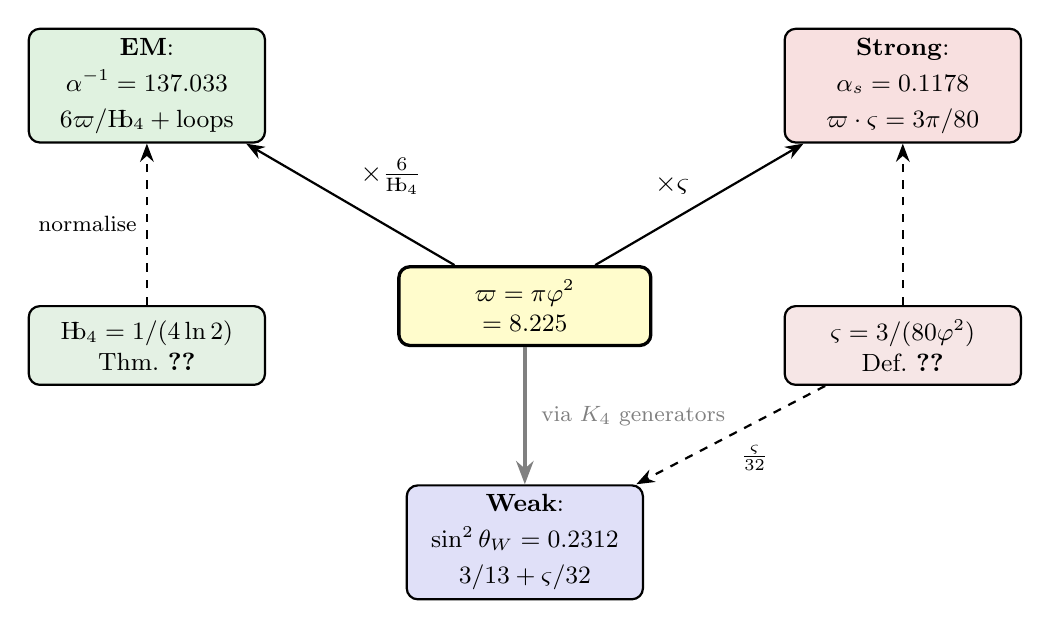
\begin{tikzpicture}[
    box/.style={draw, rounded corners, minimum width=3.0cm, minimum height=1.0cm,
                align=center, font=\small, thick},
    >=Stealth, thick
]
    % Central node — spectral bond
    \node[box, fill=yellow!20, very thick, minimum width=3.2cm] (sb) at (0,0)
        {$\specbond = \pi\varphi^2$\\$= 8.225$};

    % Three couplings
    \node[box, fill=u1color!12] (em) at (-4.8, 2.8)
        {\textbf{EM}:\\[2pt]$\alpha^{-1} = 137.033$\\[2pt]$6\specbond/\Hbfour + \text{loops}$};
    \node[box, fill=su3color!12] (strong) at (4.8, 2.8)
        {\textbf{Strong}:\\[2pt]$\alpha_s = 0.1178$\\[2pt]$\specbond \cdot \gs = 3\pi/80$};
    \node[box, fill=su2color!12] (weak) at (0, -3.0)
        {\textbf{Weak}:\\[2pt]$\sin^2\theta_W = 0.2312$\\[2pt]$3/13 + \gs/32$};

    % Supporting constants
    \node[box, fill=codegreen!12] (hb) at (-4.8, -0.5)
        {$\Hbfour = 1/(4\ln 2)$\\Thm.~\ref{S1:thm:hb4}};
    \node[box, fill=anchorcolor!12] (strain) at (4.8, -0.5)
        {$\gs = 3/(80\varphi^2)$\\Def.~\ref{S1:def:strain}};

    % Arrows — primary flows
    \draw[->] (sb) -- (em) 
        node[midway, above right, font=\normalsize] {$\times \frac{6}{\Hbfour}$};
    \draw[->] (sb) -- (strong) 
        node[midway, above left, font=\normalsize] {$\times \gs$};
    \draw[->, very thick, gray] (sb) -- (weak)
        node[midway, right=2pt, font=\footnotesize] {via $K_4$ generators};

    % Arrows — supporting
    \draw[->, thick, dashed] (hb) -- (em)
        node[midway, left, font=\footnotesize] {normalise};
    \draw[->, thick, dashed] (strain) -- (strong);
    \draw[->, thick, dashed] (strain) -- (weak)
        node[midway, below right, font=\footnotesize] {$\frac{\gs}{32}$};
\end{tikzpicture}
\caption{The QSD coupling triangle. All gauge couplings flow from the spectral bond $\specbond = \pi\varphi^2$ (centre), supported by the holographic bit density $\Hbfour$ (left) and the geometric strain $\gs$ (right). The electromagnetic coupling sums $\specbond$ over all 6 $K_4$ edges with holographic normalisation. The strong coupling multiplies $\specbond$ by strain directly. The mixing angle is a generator ratio with spectral correction.}
\label{S1:fig:coupling_triangle}
\end{figure}

%==============================================================================
\section{Summary of Axiom-to-Prediction Chain}
\label{S1:sec:summary}
%==============================================================================

\begin{center}
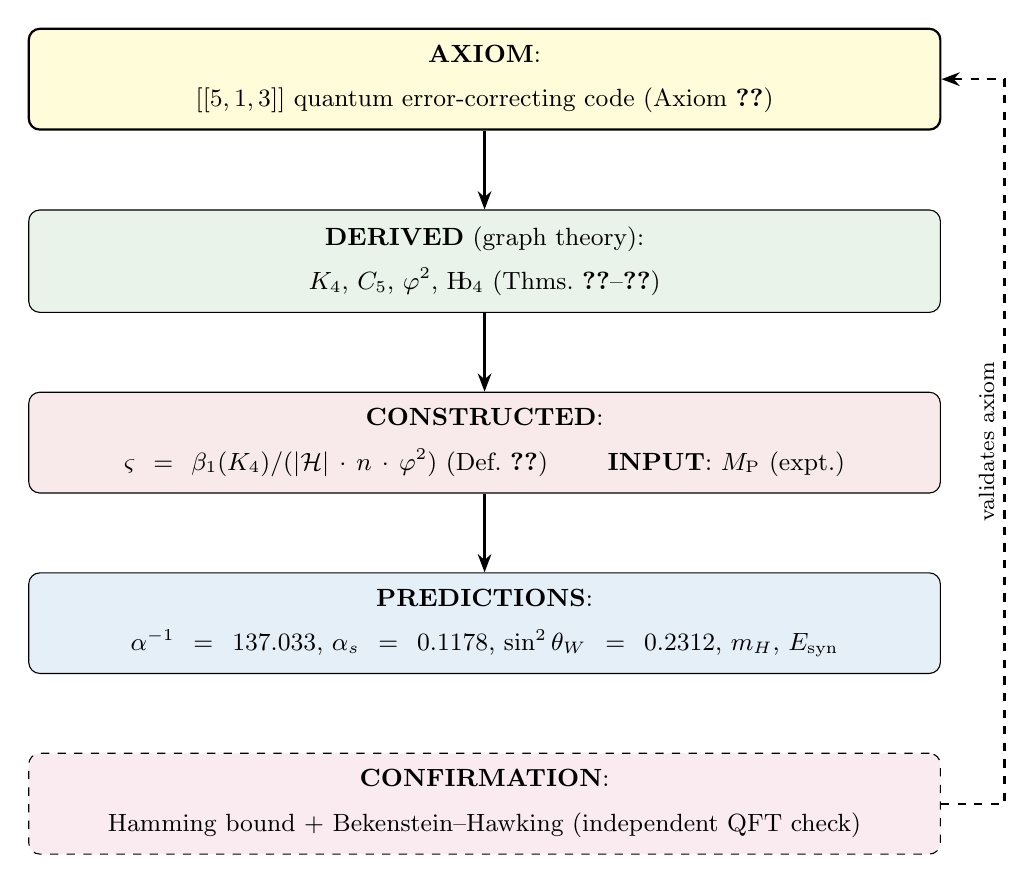
\begin{tikzpicture}[
  tier/.style={draw, rounded corners, align=center, font=\small,
               minimum height=1.25cm, text width=0.92\textwidth, inner sep=6pt},
  arrow/.style={-{Stealth}, thick},
  note/.style={font=\footnotesize},
  node distance=10mm,
]
  \usetikzlibrary{positioning,calc}

  \node[tier, fill=yellow!15, thick] (a)
    {\textbf{AXIOM}:\\[5pt] $[[5,1,3]]$ quantum error-correcting code (Axiom~\ref{S1:axiom:code})};

  \node[tier, fill=codegreen!10, below=of a] (d1)
    {\textbf{DERIVED} (graph theory):\\[5pt] $K_4$, $C_5$, $\varphi^2$, $\Hbfour$ (Thms.~\ref{S1:thm:K4}--\ref{S1:thm:hb4})};

  \node[tier, fill=anchorcolor!10, below=of d1] (p)
    {\textbf{CONSTRUCTED}:\\[5pt] $\gs = \beta_1(K_4)/(|\mathcal{H}| \cdot n \cdot \varphi^2)$ (Def.~\ref{S1:def:strain})
     \qquad \textbf{INPUT}: $\Mpl$ (expt.)};

  \node[tier, fill=bulkcolor!10, below=of p] (r)
    {\textbf{PREDICTIONS}:\\[5pt] $\alpha^{-1}=137.033$, $\alpha_s=0.1178$, $\sin^2\theta_W=0.2312$, $m_H$, $E_{\mathrm{syn}}$};

  \node[tier, fill=purple!8, dashed, below=of r] (c)
    {\textbf{CONFIRMATION}:\\[5pt] Hamming bound + Bekenstein--Hawking (independent QFT check)};

  % Main pipeline (left spine)
  \draw[arrow] (a) -- (d1);
  \draw[arrow] (d1) -- (p);
  \draw[arrow] (p) -- (r);

    % Right-side loop back to axiom (tight corridor + vertical label)
\usetikzlibrary{calc}

\coordinate (loopX) at ($(a.east)+(8mm,0)$); % reduce if still too wide, e.g. 2mm

\draw[arrow, dashed]
  (c.east) -- ++(6pt,0) coordinate (s)                 % step out of the box
  -- ($(loopX |- s)$)                                  % go to corridor x at current y
  -- ($(loopX |- a.east)$)                              % go up to axiom y (vertical segment)
      node[midway, above, rotate=90, font=\footnotesize] {validates axiom}
  -- (a.east);                                         % go left into the axiom

\end{tikzpicture}
\end{center}


%==============================================================================
% REFERENCES
%==============================================================================

\bibliographystyle{unsrt}
\bibliography{qsd_references}

\end{document}
